%%%%%%%%%%%%%%%%%%%%%%%%%%%%%%%%%%%%%%%%%
% Programming/Coding Assignment
% LaTeX Template
%
% This template has been downloaded from:
% http://www.latextemplates.com
%
% Original author:
% Ted Pavlic (http://www.tedpavlic.com)
%
% Note:
% The \lipsum[#] commands throughout this template generate dummy text
% to fill the template out. These commands should all be removed when
% writing assignment content.
%
% This template uses a Perl script as an example snippet of code, most other
% languages are also usable. Configure them in the "CODE INCLUSION
% CONFIGURATION" section.
%
%%%%%%%%%%%%%%%%%%%%%%%%%%%%%%%%%%%%%%%%%

%----------------------------------------------------------------------------------------
%	PACKAGES AND OTHER DOCUMENT CONFIGURATIONS
%----------------------------------------------------------------------------------------

\documentclass{article}

\usepackage{fancyhdr} % Required for custom headers
\usepackage{lastpage} % Required to determine the last page for the footer
\usepackage{extramarks} % Required for headers and footers
\usepackage[usenames,dvipsnames]{color} % Required for custom colors
\usepackage{graphicx} % Required to insert images
\usepackage{listings} % Required for insertion of code
\usepackage{courier} % Required for the courier font
\usepackage{lipsum} % Used for inserting dummy 'Lorem ipsum' text into the template
\usepackage[utf8]{inputenc}
\usepackage{amsmath,amssymb,amsfonts,amsthm,graphicx,enumitem}
\usepackage[parfill]{parskip}
\usepackage{color}
\usepackage{float}
\usepackage[ruled,vlined]{algorithm2e}
% Margins
\topmargin=-0.45in
\evensidemargin=0in
\oddsidemargin=0in
\textwidth=6.5in
\textheight=9.0in
\headsep=0.25in

\linespread{1.1} % Line spacing

% Set up the header and footer
\pagestyle{fancy}
\lhead{\hmwkAuthorName} % Top left header
\chead{\hmwkClass\ (\hmwkClassInstructor\ \hmwkClassTime): \hmwkTitle} % Top center head
\rhead{\firstxmark} % Top right header
\lfoot{\lastxmark} % Bottom left footer
\cfoot{} % Bottom center footer
\rfoot{Page\ \thepage\ of\ \protect\pageref{LastPage}} % Bottom right footer
\renewcommand\headrulewidth{0.4pt} % Size of the header rule
\renewcommand\footrulewidth{0.4pt} % Size of the footer rule

\setlength\parindent{0pt} % Removes all indentation from paragraphs

%----------------------------------------------------------------------------------------
%	CODE INCLUSION CONFIGURATION
%----------------------------------------------------------------------------------------

\definecolor{MyDarkGreen}{rgb}{0.0,0.4,0.0} % This is the color used for comments
\lstloadlanguages{Perl} % Load Perl syntax for listings, for a list of other languages supported see: ftp://ftp.tex.ac.uk/tex-archive/macros/latex/contrib/listings/listings.pdf
\lstset{language=Perl, % Use Perl in this example
        frame=single, % Single frame around code
        basicstyle=\small\ttfamily, % Use small true type font
        keywordstyle=[1]\color{Blue}\bf, % Perl functions bold and blue
        keywordstyle=[2]\color{Purple}, % Perl function arguments purple
        keywordstyle=[3]\color{Blue}\underbar, % Custom functions underlined and blue
        identifierstyle=, % Nothing special about identifiers
        commentstyle=\usefont{T1}{pcr}{m}{sl}\color{MyDarkGreen}\small, % Comments small dark green courier font
        stringstyle=\color{Purple}, % Strings are purple
        showstringspaces=false, % Don't put marks in string spaces
        tabsize=5, % 5 spaces per tab
        %
        % Put standard Perl functions not included in the default language here
        morekeywords={rand},
        %
        % Put Perl function parameters here
        morekeywords=[2]{on, off, interp},
        %
        % Put user defined functions here
        morekeywords=[3]{test},
       	%
        morecomment=[l][\color{Blue}]{...}, % Line continuation (...) like blue comment
        numbers=left, % Line numbers on left
        firstnumber=1, % Line numbers start with line 1
        numberstyle=\tiny\color{Blue}, % Line numbers are blue and small
        stepnumber=5 % Line numbers go in steps of 5
}

% Creates a new command to include a perl script, the first parameter is the filename of the script (without .pl), the second parameter is the caption
\newcommand{\perlscript}[2]{
\begin{itemize}
\item[]\lstinputlisting[caption=#2,label=#1]{#1.pl}
\end{itemize}
}

%----------------------------------------------------------------------------------------
%	DOCUMENT STRUCTURE COMMANDS
%	Skip this unless you know what you're doing
%----------------------------------------------------------------------------------------

% Header and footer for when a page split occurs within a problem environment
\newcommand{\enterProblemHeader}[1]{
\nobreak\extramarks{#1}{#1 continued on next page\ldots}\nobreak
\nobreak\extramarks{#1 (continued)}{#1 continued on next page\ldots}\nobreak
}

% Header and footer for when a page split occurs between problem environments
\newcommand{\exitProblemHeader}[1]{
\nobreak\extramarks{#1 (continued)}{#1 continued on next page\ldots}\nobreak
\nobreak\extramarks{#1}{}\nobreak
}

\setcounter{secnumdepth}{0} % Removes default section numbers
\newcounter{homeworkProblemCounter} % Creates a counter to keep track of the number of problems

\newcommand{\homeworkProblemName}{}
\newenvironment{homeworkProblem}[1][Problem \arabic{homeworkProblemCounter}]{ % Makes a new environment called homeworkProblem which takes 1 argument (custom name) but the default is "Problem #"
\stepcounter{homeworkProblemCounter} % Increase counter for number of problems
\renewcommand{\homeworkProblemName}{#1} % Assign \homeworkProblemName the name of the problem
\section{\homeworkProblemName} % Make a section in the document with the custom problem count
\enterProblemHeader{\homeworkProblemName} % Header and footer within the environment
}{
\exitProblemHeader{\homeworkProblemName} % Header and footer after the environment
}

\newcommand{\problemAnswer}[1]{ % Defines the problem answer command with the content as the only argument
\noindent\framebox[\columnwidth][c]{\begin{minipage}{0.98\columnwidth}#1\end{minipage}} % Makes the box around the problem answer and puts the content inside
}

\newcommand{\homeworkSectionName}{}
\newenvironment{homeworkSection}[1]{ % New environment for sections within homework problems, takes 1 argument - the name of the section
\renewcommand{\homeworkSectionName}{#1} % Assign \homeworkSectionName to the name of the section from the environment argument
\subsection{\homeworkSectionName} % Make a subsection with the custom name of the subsection
\enterProblemHeader{\homeworkProblemName\ [\homeworkSectionName]} % Header and footer within the environment
}{
\enterProblemHeader{\homeworkProblemName} % Header and footer after the environment
}

%----------------------------------------------------------------------------------------
%	NAME AND CLASS SECTION
%----------------------------------------------------------------------------------------

\newcommand{\hmwkTitle}{Assignment\ \#3} % Assignment title
\newcommand{\hmwkDueDate}{} % Due date
\newcommand{\hmwkClass}{NPDE for Option Pricing } % Course/class
\newcommand{\hmwkClassTime}{12:20am} % Class/lecture time
\newcommand{\hmwkClassInstructor}{Instructor:Dr.Kopriva} % Teacher/lecturer
\newcommand{\hmwkAuthorName}{Jian Wang } % Your name

%----------------------------------------------------------------------------------------
%	TITLE PAGE
%----------------------------------------------------------------------------------------

\title{
\vspace{2in}
\textmd{\textbf{\hmwkClass:\ \hmwkTitle}}\\
\normalsize\vspace{0.1in}\small{Due\ on\ \hmwkDueDate}\\
\vspace{0.1in}\large{\textit{\hmwkClassInstructor\ \hmwkClassTime}}
\vspace{3in}
}

\author{\textbf{\hmwkAuthorName}}
\date{} % Insert date here if you want it to appear below your name

%----------------------------------------------------------------------------------------

\begin{document}

\maketitle

%----------------------------------------------------------------------------------------
%	TABLE OF CONTENTS
%----------------------------------------------------------------------------------------

%\setcounter{tocdepth}{1} % Uncomment this line if you don't want subsections listed in the ToC

\newpage
\tableofcontents
\newpage

%% insert the programming code
%\begin{homeworkProblem}
%Listing \ref{homework_example} shows a Perl script.
%
%\perlscript{homework_example}{Sample Perl Script With Highlighting}
%
%\lipsum[1]
%\end{homeworkProblem}

%% insert the chart
%\begin{homeworkProblem}
%\lipsum[2]
%
%\problemAnswer{
%\begin{center}
%\includegraphics[width=0.75\columnwidth]{example_figure} % Example image
%\end{center}
%\lipsum[3-5]
%}
%\end{homeworkProblem}
%% Example of list array and emurate
%\begin{homeworkProblem}
%
%\begin{flalign}
%A =
%\begin{bmatrix}
%A_{11} & A_{21} \\
%A_{21} & A_{22}
%\end{bmatrix}
%\end{flalign}
%
%\begin{itemize}
%	\item First item in a list
%		\begin{itemize}
%		\item First item in a list
%			\begin{itemize}
%			\item First item in a list
%			\item Second item in a list
%			\end{itemize}
%		\item Second item in a list
%		\end{itemize}
%	\item Second item in a list
%\end{itemize}
%
%\begin{enumerate}
%\item First item in a list
%\item Second item in a list
%\item Third item in a list
%\end{enumerate}

%% equation formula
%$\left \{
%\begin{tabular}{l}
%$V_t+\frac{\sigma^2S^2}{2}V_{SS}+rSV_s - rV=0$\\
%
%$V(0,t)=e^{-r(T-t)}$\\
%
%$V(\infty,t)=0$\\
%
%$V(S,T)=I_{\{S\leq K\}}$
%\end{tabular}
%\right.$

%\end{homeworkProblem}
%----------------------------------------------------------------------------------------

\begin{homeworkProblem}

\section*{[Summary]}
1) CPU time for the ADI algorithms doubled when time meshes doubled and quadrupled when stock meshes quadrupled. The value of the option was 0.2459.\\

2) When the stock 1 price or stock 2 price was equal to 0 , we treated the boundary conditions as the one dimensional European put option problem and used the Black Scholes formula to calculated the option prices.\\

3) The main idea of the ADI method was to proceed in two stages, treating only one operator implicitly at
each stage. For this rainbow option problem, the implementation of ADI algorithm was not easy and some papers showed that it was not as efficient as Operator splitting method.\\

\section*{[Statement of the problem]}
In this assignment, we need to calculate the price of rainbow option with the price of the maximum of two risky assets. We try to compute the option for the parameters K = 100, T = 0.25, r = 0.15, $\sigma_1$ = 0.15, $\sigma_2$ =0.20, and $\rho$= -0.20. Our task is to report the value of the option based on those assumptions. \\

We choose the Alternating Direction Implicit (ADI) method to solve the linear system. \\

In this report, we also report the CPU time that is needed to get the solutions on a 128 X 128 point mesh. These times will be used to compare the methods among classmates. We also explain the choices that we have made and how they affect our solutions and computational efficiency.\\


\section*{[Description of The Mathematics]}
\textbf{PDE formula}
The BSM and boundary condition for the Rainbow European put option is:\\
\begin{flalign*}
V_t+\frac{1}{2}\sigma_1^2S_1^2V_{S_1S_1}+\frac{1}{2}\sigma_1^2S_2^2V_{S_2S_2}+rS_1V_{S_1}+rS_2V_{S_2}+\rho\sigma_1\sigma_2S_1S_2V_{S_1S_2}-rv =0
\end{flalign*}
\\
Where the payoff function is: \\
\begin{flalign*}
V(S_1, S_2,T ) = max (K-max(S_1,S_2),0)
\end{flalign*}

\textbf{[Analytical solution of the Rainbow put option:]\\}
From the paper "R.M.Stulz. Options on the minimum or the maximum of two risky assets, Journal of Financial Economics, 10:161 - 185, February, 1982), we can find the exact solution of the Rainbow European put option.\\

In his paper: \\
$F$: represented the strike price.\\
$V$: represented one stock price.\\
$H$: represented the other stock price.\\
$R$: is the interest rate.\\
$\tau=T-t$: was the time remaining to the maturity.\\
$\sigma_H$: was the volatility of stock H.\\
$\sigma_V$: was the volatility of stock V.\\

The price of a put option on the maximum of two risky assets was:\\

$PX(V,H,F,\tau)=e^{-R\tau}F-MX(V,H,0,\tau)+MX(V,H,F,\tau)$\\

Where $PX(V.H,F,\tau)$ is a European put option on the maximum of asset V and H with strike price F and time to maturity $\tau$.\\
$MX(V,H,F,\tau)=C(V,F,\tau)+C(H,F,\tau)-M(V,H,F,\tau)$\\
Where, $C(A,F,\tau)$ was an European call option on asset A with strike price F.\\

$M(V,H,F,\tau)=HN_2(\gamma_1\sigma_H\sqrt{\tau},(ln(V/H)-0.5*\sigma^2\tau/\sigma\sqrt{\tau},(\rho_{VH}\sigma_V-\sigma_H)/\sigma)+VN_2(\gamma_2\sigma_V\sqrt{\tau},(ln(H/V)-0.5*\sigma^2\tau/\sigma\sqrt{\tau},(\rho_{VH}\sigma_H-\sigma_V)/\sigma)-Fe^{-r\tau}N_2(\gamma_1,\gamma_2,\rho_{VH})$\\

Where:\\$\gamma_1=(ln(H/F)+(R-0.5*\sigma^2_H)\tau)/(\sigma_H*\sqrt{\tau})$\\
$\gamma_2=(ln(V/F)+(R-0.5*\sigma^2_V)\tau)/(\sigma_V*\sqrt{\tau})$\\
$\sigma^2=\sigma_V^2+\sigma_H^2-2\rho_{VH}\sigma_V\sigma_H$\\

\section*{[Description of Algorithm]}

The algorithm to solve the rainbow put option was as follows:\\
$\frac{u_{ij}^{n+1}-u_{ij}^n}{\Delta \tau}=L_{ADI}^xu_{ij}^{n+1/2}+L_{ADI}^yu_{ij}^{n+1}$\\

\textbf{step 1:} \\
The ADI method equation can be rewritten as:\\

$\alpha_iu_{i-1,j}^{n+1/2}+\beta_iu_{ij}^{n+1/2}+\gamma_iu_{i+1,j}^{n+1/2}=f_{ij}$\\

Where: \\

$\alpha_i=-\frac{(\sigma_1x_i)^2}{4h^2}$\\

$\beta_i=\frac{1}{\Delta \tau}+\frac{(\sigma_1x_i)^2}{2h^2}+\frac{rx_j}{2h}\frac{r}{2}$\\

$f_{ij}=\frac{u_{ij}^n}{\Delta \tau}+\frac{1}{4}(\sigma_2 y_j)^2\frac{u_{i,j+1}^n-2u_{ij}^n+u_{i,j-1}^n}{h^2}+
\frac{1}{2}\rho\sigma_1 \sigma_2 x_i y_j\frac{u_{i+1,j+1}^n+u_{i-1,j-1}^n-u_{i-1,j+1}^n-u_{i+1,j-1}^n}{4h^2}$


So we can get the $A_x$ as a tridiagonal matrix constructed from the above equation.\\

\begin{flalign*}
A_x =
\begin{Bmatrix}
2\alpha_0+\beta_0&\gamma_0-\alpha_0 &0&\cdots&0&0 \\
\alpha_1&\beta_1&\gamma_1&\cdots&0&0\\
0&\alpha_2&\beta_w&\cdots&0&0\\
\vdots&\vdots&\ddots&\ddots&\ddots&\vdots\\
0&0&0&\cdots&\beta_{N_x-1}&\gamma_{N_x-1}\\
0&0&0&\cdots&\alpha_{N_x}-\gamma_{N_x}&\beta_{N_x}+2\gamma_{N_x}\\
\end{Bmatrix}
\end{flalign*}

The calculation algorithm was as follows:\\
$1:for\ j = 0: N_y$\\
$2:\quad$$ for\ i = 0:N_x$\\
$3:\quad \quad Set\ \alpha_i,\beta_i,\gamma_i\ and\ f_ij$\\
$4:\quad end$\\
$5:\quad Solve\ A_xu_{0:N_x,j}^{n+1/2}=f_{0:N_x,j}\ by\ PSOR \  method$\\
$6:end$

\textbf{step2:}\\

$\alpha_ju_{i,j-1}^{n+1}+\beta_ju_{ij}^{n+1}+\gamma_ju_{i,j+1}^{n+1}=g_{ij}$\\

Where: \\
$\alpha_j=-\frac{(\sigma_2y_j)^2}{4h^2}$\\

$\beta_j=\frac{1}{\Delta \tau}+\frac{(\sigma_2y_j)^2}{2h^2}+\frac{ry_j}{2h}+\frac{r}{2}$\\

$g_{ij}=\frac{u_{ij}^{n+1/2}}{\Delta \tau}+\frac{1}{4}(\sigma_1 x_i)^2\frac{u_{i+1,j}^{n+1/2}-2u_{ij}^{n+1/2}+u_{i-1,j}^{n+1/2}}{h^2}+\frac{1}{2}rx_i\frac{u_{i+1,j}^{n+1/2}-u_{i,j}^{n+1/2}}{h}
+\frac{1}{2}\rho\sigma_1 \sigma_2 x_iy_j\frac{u_{i+1,j+1}^{n+1/2}+u_{i-1,j-1}^{n+1/2}-u_{i-1,j+1}^{n+1/2}-u_{i+1,j-1}^{n+1/2}}{4h^2}$


So we can get the $A_y$ as a tridiagonal matrix constructed from the above equation.\\

\begin{flalign*}
A_y =
\begin{Bmatrix}
2\alpha_0+\beta_0&\gamma_0-\alpha_0 &0&\cdots&0&0 \\
\alpha_1&\beta_1&\gamma_1&\cdots&0&0\\
0&\alpha_2&\beta_w&\cdots&0&0\\
\vdots&\vdots&\ddots&\ddots&\ddots&\vdots\\
0&0&0&\cdots&\beta_{N_y-1}&\gamma_{N_y-1}\\
0&0&0&\cdots&\alpha_{N_y}-\gamma_{N_y}&\beta_{N_y}+2\gamma_{N_y}\\
\end{Bmatrix}
\end{flalign*}

The calculation algorithm was as follows:\\
$1:for\ i = 0: N_x$\\
$2:\quad$$ for\ j = 0:N_y$\\
$3:\quad \quad Set\ \alpha_j,\beta_j,\gamma_j\ and\ g_{ij}$\\
$4:\quad end$\\
$5:\quad Solve\ A_yu_{i,0:N_y}^{n+1}=g_{i,0:N_y}\ by\ PSOR \  method$\\
$6:end$

\section*{numerical results:}
\textbf{[Boundary conditions:]}\\
We chose the following boundary conditions:\\

1)When Time to maturity was equal to 0 :\\
The boundary condition was the value payoff function based on $S_1$, $S_2$, and K. \\
$Payoff= max(K-max(S_1,S_2),0)$\\
The following chart showed this boundary condition.\\
\begin{center}
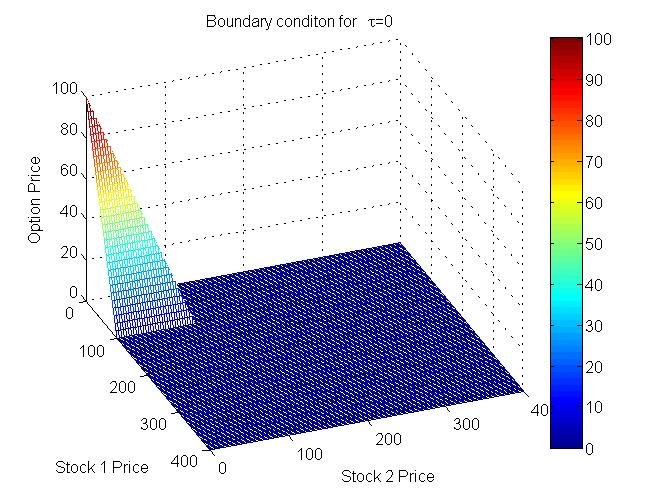
\includegraphics[width=0.75\columnwidth]{t.jpg} % Example image
\end{center}

2) When stock price 1 was equal to zero.\\
The boundary condition was set to be the one dimensional European put option based on $S_2$, $K$,$\sigma_2$,$r$, and $T$. We used the Black Scholes formula to calculated the price of European put option.The following chart demonstrated this boundary condition.\\
\begin{center}
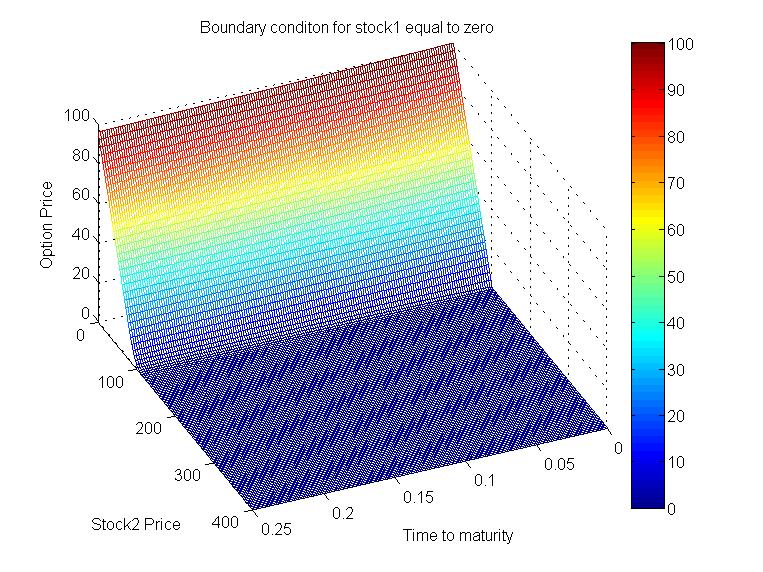
\includegraphics[width=0.75\columnwidth]{b1.jpg} % Example image
\end{center}

3) When stock price 2 was equal to zero.\\
The boundary condition was set to be the one dimensional European put option based on $S_1$, $K$,$\sigma_1$,$r$, and $T$. The following chart demonstrated this boundary condition.\\
\begin{center}
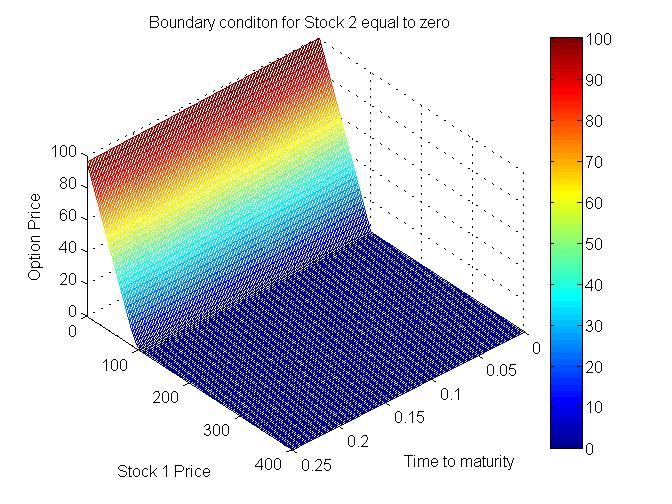
\includegraphics[width=0.75\columnwidth]{b2.jpg} % Example image
\end{center}

4) When stock price 1 or stock price 2  was equal to 4 times strike price.\\
The boundary condition here was set to be the 0;

\textbf{Results and CPU times}

We set the stock meshes to be 128x128 and 256 x 256, and changed the time meshes from 40 to 640, doubled each time.\\
The following table listed the results of the CPU time.\\
\begin{center}
\begin{tabular}{|ccc|}
\hline
 & CPU Time(S)& \\
\hline
Time meshes& Stock meshes(128x128)&  Stock meshes(256x256)\\
40&3.26847&17.18241\\
80&5.603745&29.245583\\
160&10.716801&48.744667\\
320&20.84432&87.875921\\
640&45.651938&152.364333\\
\hline
\end{tabular}
\end{center}

The value of the option price was 0.2459 and the following two charts showed the analytical solutions and numerical solutions for the European rainbow put options based on different stock 1 and stock 2 prices.\\
Analytical solutions surfaces:\\
\begin{center}
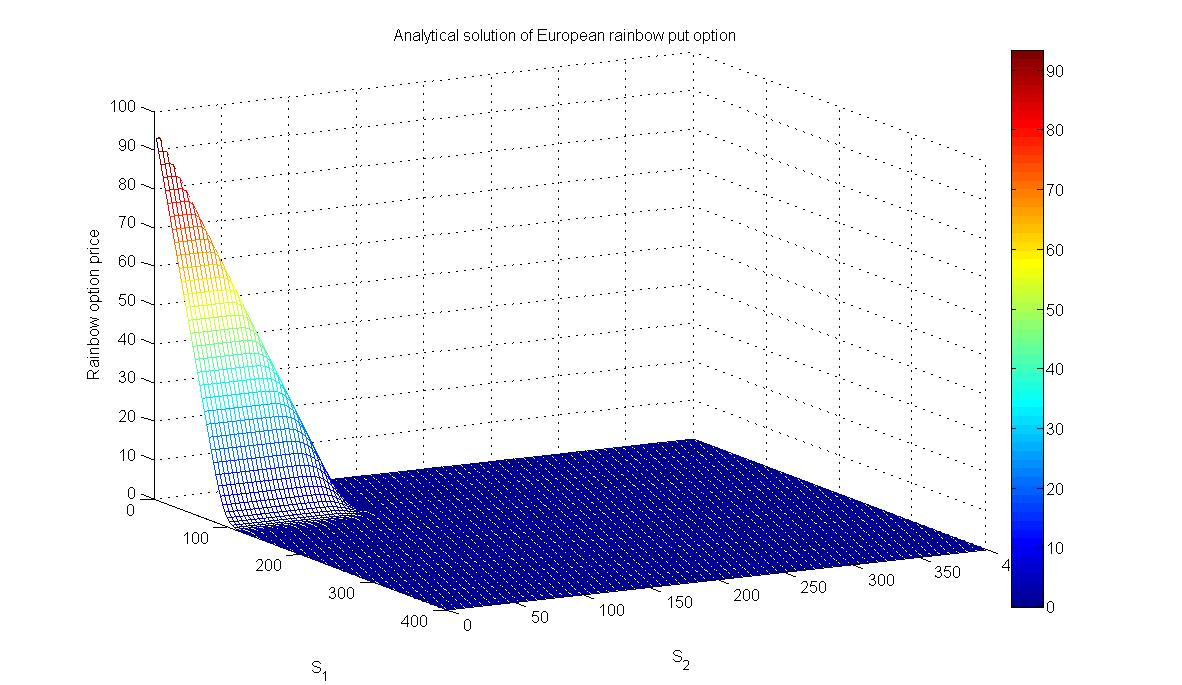
\includegraphics[width=0.75\columnwidth]{close.jpg} % Example image
\end{center}
Numerical solutions(ADI) surfaces:\\
\begin{center}
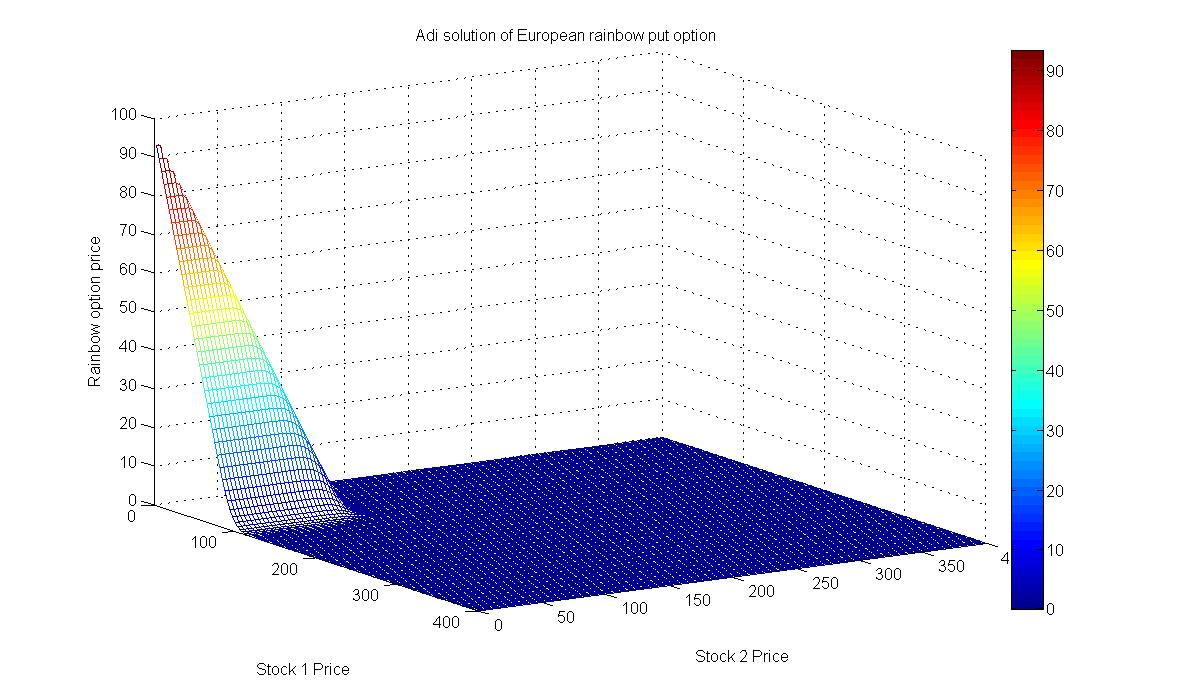
\includegraphics[width=0.75\columnwidth]{adi.jpg} % Example image
\end{center}

\end{homeworkProblem}
\end{document} 